\chapter{PAWS - Towards PIPS as Web Service}

This first chapter introduces the idea of creating PaWS framework. It
answers two questions: why it is needed? and on what it is based? Design
constraints and functional requirements also are presented here. They
resulted in the emergence of three main modes for PaWS. They are
described in the next section (?). The last part of this chapter presents
the creation process of PaWS.

\section{PaWS}

The introduction page presents overall information about PaWS and PIPS in the panel on the left side, as it is shown in the Figure \ref{fig:intro_page}.

\begin{figure}[h!]
  \centering
  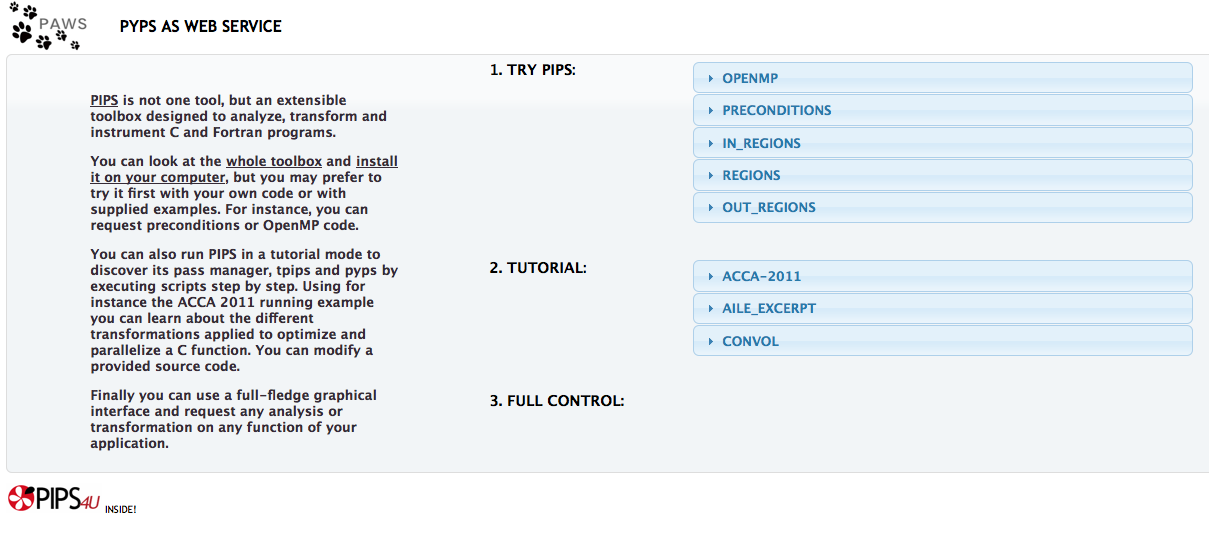
\includegraphics[width=0.8\textwidth]{reportCh4/intro_page}
  \caption{PaWS Introduction page.}
  \label{fig:intro_page}
\end{figure}

Left side panel allows the user to choose mode and its concrete tool or demonstration. To do it, the user has to click on the tab of the chosen tool/demonstration. It will be expanded (see Figure \ref{fig:expanded_tab}) with more detailed information and links to the actual sites visible.

\begin{figure}[h!]
  \centering
  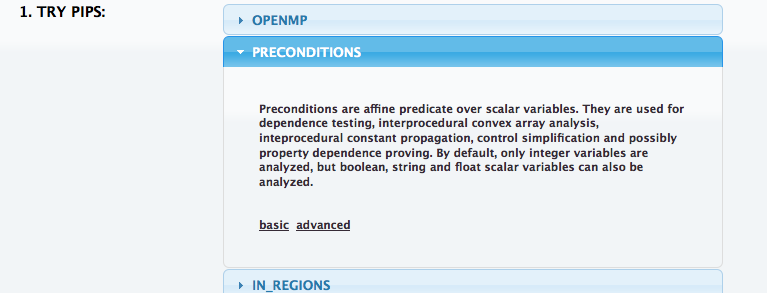
\includegraphics[width=1.0\textwidth]{reportCh4/expanded_tab}
  \caption{Expanded preconditions tab.}
  \label{fig:expanded_tab}
\end{figure}

To come back to the introduction page, the user can use logo image (see Figure \ref{fig:logo_image}) as a link.

\begin{figure}[h!]
  \centering
  
\includegraphics[width=0.2\textwidth]{reportCh4/logo_image}
  \caption{Logo image as home page link.}
  \label{fig:logo_image}
\end{figure}
\section{Design constraints}
\label{design_contraints}

As explained in the previous section, the main goal of the PaWS
framework is to create a very light WEB interface for PIPS. But PaWS is also
subjected to other, more detailed constraints:

\begin{enumerate}

  \item {\bf No installation requirements} on a the client side, beyond
  a browser.

  \item {\bf PIPS scripting complexity is hidden}: the result of any
    operation is displayed in a source form thru a few clicks.

  \item {\bf Separation of PIPS, PyPS and PaWS}: to avoid dependencies
    between pieces of software and to protect the WEB server from crashes
    caused by PIPS internal errors.

  \item {\bf Easy customization of PaWS}: PIPS developers, who are not
    familiar with PaWS and Pylons, should be able to update the PaWS
    configuration and add new passes or tutorials. 

    % Process of changing particular element is easy, because
    % application is based on the structure of the files which
    % contains python modules with pyps functionalities, examples and
    % files with descriptions of them.

  \item {\bf PIPS server is up-to-date}: use a recent version of PIPS,
    that is properly validated.

  \item {\bf Security}: against spamming engines, it is obtained by
    forbidding Python or shell input and by using a login and a
    password.

  \item {\bf Consistency} between:
    \begin{itemize}
      \item the output computed by Tpips and by Pyps;
      \item the output of the cut-and-pasted code, code loaded from
        the PaWS example, code loaded from the user machine and
        modified code.
    \end{itemize}

  \item {\bf Use PIPS validation mechanism to validate PaWS
      configuration}

  \item {\bf Protection against server overload}: assure PaWS
    availability; control response time.

  \item {\bf Code Reuse}: use existing components as much as possible
    and a generic approach to page creation.

  \item {\bf OS neutrality}

\end{enumerate}

%%  \item {\bf remote execution of PIPS -> demo? not sure}

\section{Design Requirements}
\label{design_requirements}

PaWS framework has several functional requirements, some times related
to the design constraints:

\begin{enumerate}

  \item {\bf Uploading user files (also multiple
      files)}\label{req:uploading_files}: user can provide the source
    code not only by typing or copy-and-pasting it into the
    application window, but also by browsing and picking it from
    his/her machine.

  \item {\bf Saving results on user
      machine}\label{req:saving_results}: user can write back the
    result of the analysis or transformation as a file on his/her
    machine.

  \item {\bf Printing results}\label{req:printing_results}: the user can
    print the result of the analysis or transormation on his/her
    printer.

  \item {\bf Presenting dependence
      graphs}\label{req:dependence_graphs}: user can create and
    display dependence graph of his/her source code. Also
    demonstrations can include graphs.

  \item {\bf Detecting language}\label{req:language_detection}:
    programming language of the source code is detected and
    displayed. C, Fortran77 and, to some extent, Fortran 90 are supported.

  \item {\bf Deleting temporary files}\label{req:deleting_files}:
    temporary files, which are not used anymore, are removed from the
    server disk space.

  \item {\bf Providing ready-to-use examples}\label{req:providing_examples}:
    each analysis and transformation has a set of pedagogical
    examples ready to use by the user.

  \item {\bf Authentication mechanism}\label{req:authentication}:
    access to the PaWS is protected by a simple authentication
    mechanism, a login name and a password.

\end{enumerate}

\section{PaWS Project}
\label{paws_project}

PaWS provides three different modes of using PIPS: tutorial,
elementary analysis or transformation, and full control. Each of them
presents different ways to see how PIPS is working, according to
the user needs.

%% see Introduction for goals
%% implementation vs configuration

\subsection{Tutorial mode}

Tutorial is the PaWS mode that presents PIPS pass managers to users who
are not familiar with this framework. It is also very easy way to
learn how PIPS is working. The user needs only to choose an example
and after it is loaded, he/she can follow transformations and analyses
step-by-step. The user can also skip some steps or go back to previous
ones. There is always a script and its results are presented with some
explanations. The result may include dependence graphs for pedagogical
reasons.

\subsection{Basic analyses and transformations}

This mode enables intermediate users to try specific PIPS
transformations and analysis. The user can choose prepared examples or
use his own code to see how PIPS works. He can later modify the source
code to see differences in results. PIPS related analyses and
transformations are available at two levels: basic and advanced. Basic
level performs operations with default PIPS properties. The advanced
level provides list of properties, that can be modified by the user to
obtain more accurate results or ot speed up PIPS. More information can
be found in the configuration chapter (see Section~\ref{currentconfiguration}).

\subsection{Full control}

Full control is the mode that enables users to create graphically PyPS
or TPIPS scripts which are applied later to the source code.

This mode has not been implemented yet.

\section{PaWS Development Process}

PaWS framework was created with a Agile Methodology
\cite{agilemethodology}. The whole process was made of several short iterations,
each adding new capabilities to PaWS. Each iteration had its
own list of the requirements refering to the general PaWS design
requirements and constraints (see Sections \ref{design_contraints} and
\ref{design_requirements}). After completing an iteration, it was
summed up and, according to its result, the main goals might have been
slightly modified. The list of the encountered problems is given in Section
\ref{encountered_problems}.

The goal of the first iteration was to create working skeleton of the
framework, which was linking Pylons and Pyps technologies together. It
could only perform \emph{preconditions} analysis. The next steps
included the addition of
new PIPS passes and the customization of WEB pages with
user-friendly features such as saving, printing results, and source code
colorization. Further action was to extend PaWS with the second mode -
demonstration and by possibility of creating graphs.

At the same time, consistency and stability of the PaWS framework (see Section \ref{encountered_problems}) has been being improved.

The goal of the last step of the project was to improve the existing
framework by writing tests, scripts for administrators to add new tool
or demo, refactor code and framework structure, and implementing
several user-friendly features such as the uploading of an
archive file. PaWS also was included in the PIPS building process.

%% TO DO: About process of creating PaWS application - from what we started, what was added, what was not good idea.
%% trial and error process
%% no ... agile programming
%% V CYCLE, AGILE

%% exploratory process, agile development, validation, evaluation




\section{Conclusion}

PaWS is a lightweight and easy to use application, although it refers to a very complex toolkit, which is PIPS. Design contraints and requirements which were evolving over the time and also different modes of using this framework with significant amount of examples resulted in necessity of providing flexibility in configuring and changing PaWS. It required using good architectural solution and proven tools or libraries. These issues are described in subsequent chapters.

``Web service'' in the PaWS acronim should not be taken literally. It is not the implementation of the Web Service standard \cite{ws_standard}. PaWS framework idea refers to the conception of the service\footnote{Service is the independent software element which shares complete, reusable  functionality through the well defined interface \cite{service_def}.} in general. The term ``web'' in this case means that functionality shared by the PaWS service is available via the Internet.
